%\begin{figure}[h]
%\centering
%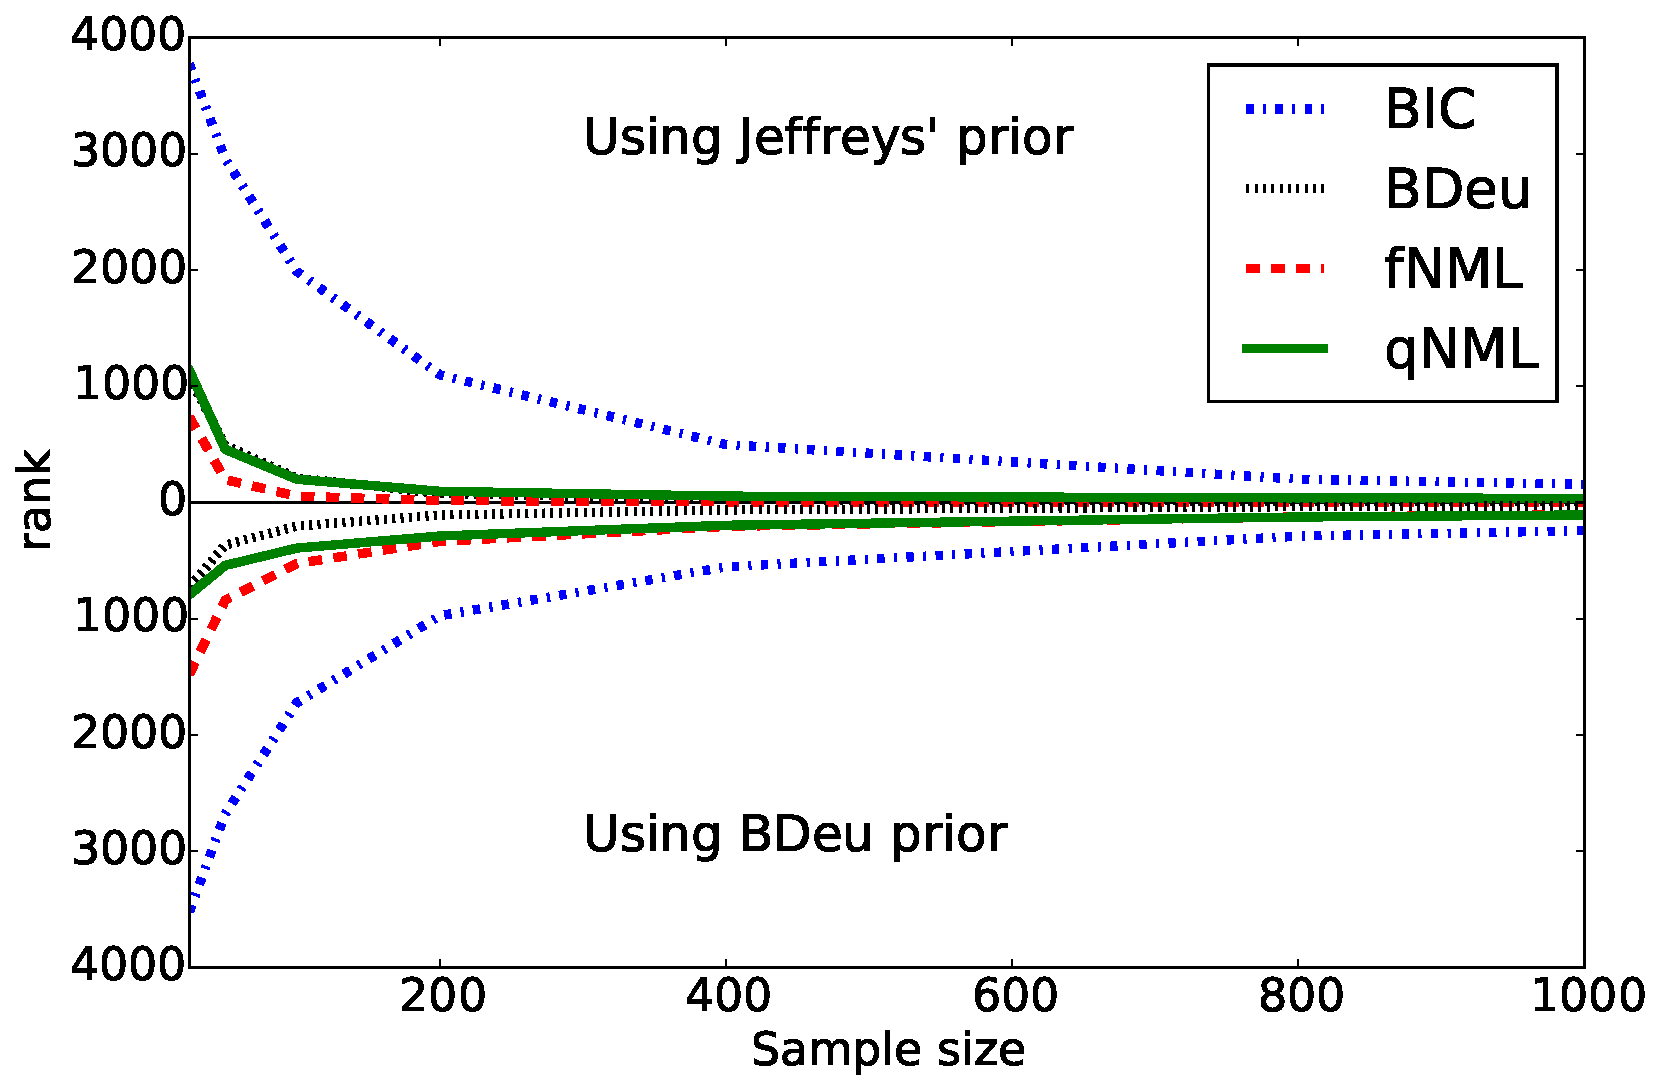
\includegraphics[width=8cm,height=5cm]{qNML_images/art4_mean.pdf}
%\caption{Finding generating models of 4 arcs.}
%\label{fig:4arcs}
%\end{figure}
\section{EXPERIMENTAL RESULTS}

We empirically compare the capacity of qNML to that of BIC, BDeu ($\alpha = 1$) and
fNML in identifying the data generating structures, and producing
models that are predictive and parsimonious.  It seems that none of
the criteria uniformly outperform the others in all these desirable
aspects of model selection criteria.

\subsection{Finding Generating Structure}

In our first experiment, we took five widely used benchmark Bayesian networks\footnote{Bayesian Network Repository: \url{http://www.bnlearn.com/bnrepository/}}, sampled data from them, and tried to learn the generating structure with the different scoring functions using various sample sizes. We used the following networks: Asia ($n=5$, 8 arcs), Cancer ($n=5$, 4 arcs), Earthquake ($n=5$, 4 arcs), Sachs ($n=11$, 17 arcs) and Survey ($n=6$, 6 arcs). These networks were picked in order to use the dynamic programming based exact structure learning~\cite{cosco.uai06} which limited the number $n$ of variables
to less than 20. We measured the quality of the learned structures using structural Hamming distance (SHD) \cite{Tsamardinos2006}.

Figure \ref{fig:all_shd} shows SHDs for all the scoring criteria for each network. Sample sizes range from $10$ to $10000$ and the shown results are averages computed from $1000$ repetitions. None of the scores dominates in all settings considered. BIC fares well when the sample size is small as it tends to produce a nearly empty graph which is a good answer in terms of SHD when the generating networks are relatively sparse. qNML obtains strong results in the Earthquake and Asia networks, being the best or the second best with all the sample sizes considered.

\begin{figure}[h]
\centering
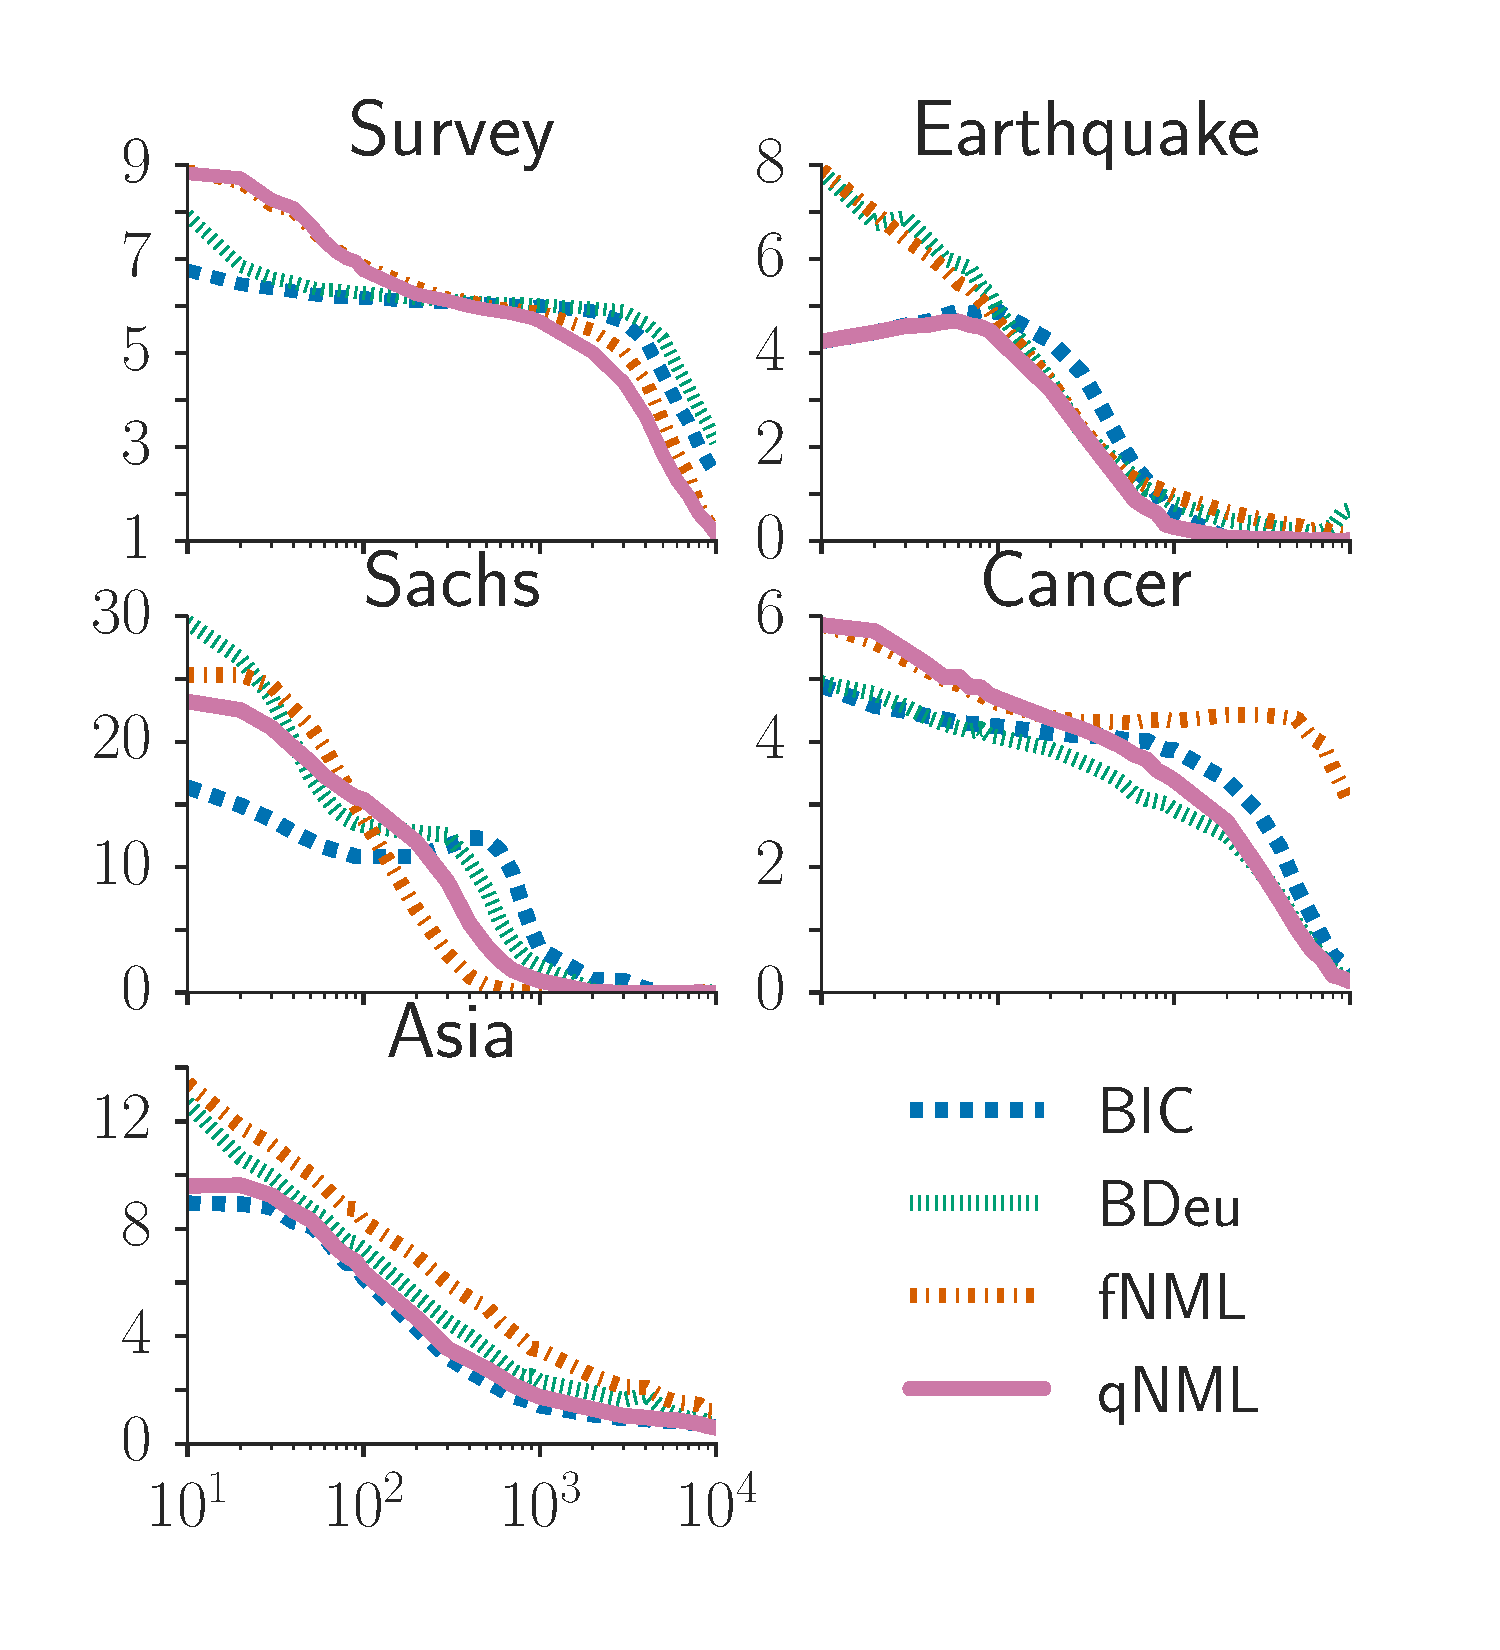
\includegraphics[width=\columnwidth]{qNML_images/shd_all.pdf}
\caption{Sample size versus SHD with data generated from real world DAGs.}
\label{fig:all_shd}
\end{figure}

Figure \ref{fig:shd_ranks} summarizes the SHD results in all networks by showing the average rank for each score. The ranking was done by giving the score with the lowest SHD rank $1$ and the worst one rank $4$. In case of ties, the methods with the same SHD were given the same rank. The shown results are averages computed from $5000$ values ($5$ networks, $1000$ repetitions). From this, we can see that qNML never has the worst average ranking, and it has the best ranking with sample sizes greater than $300$. This suggests that qNML is overall a safe choice in structure learning, especially with moderate and large sample sizes.

%We first compare the ability of the different scoring criteria to
%discover the structure that generated the data. For this purpose we
%create 100 random 5-node Bayesian network structures with 4
%edges and another 100 structures with 7 edges.  The variables were
%randomly assigned to have 2 -- 4 values ($r_i \in \{2, 3, 4\}$). For
%each network, we generated parameters by two different schemes. The
%first scheme exactly matched the assumptions of the BDeu score with
%$\alpha = 1$, i.e., the parameters were distributed by $\theta_{ij}
%\sim Dir(\frac{1}{r_iq_i},\ldots,\frac{1}{r_iq_i})$. The other scheme
%was to generate the parameters independently from a Dirichlet
%distribution $\theta_{ij} \sim Dir(\frac{1}{2},\ldots, \frac{1}{2})$
%that is the Jeffreys' prior for the multinomial model. This distribution
%was selected instead of the uniform distribution in order to make the
%generating structure more identifiable.  For each network (structure +
%parameters), we generated 100 data sets of 1000 data vectors, and
%studied how different scoring criteria ranked, on average, the structure of the
%generating network among all the 5-node networks as a function of
%(sub)sample size.

\begin{figure}[h]
\centering
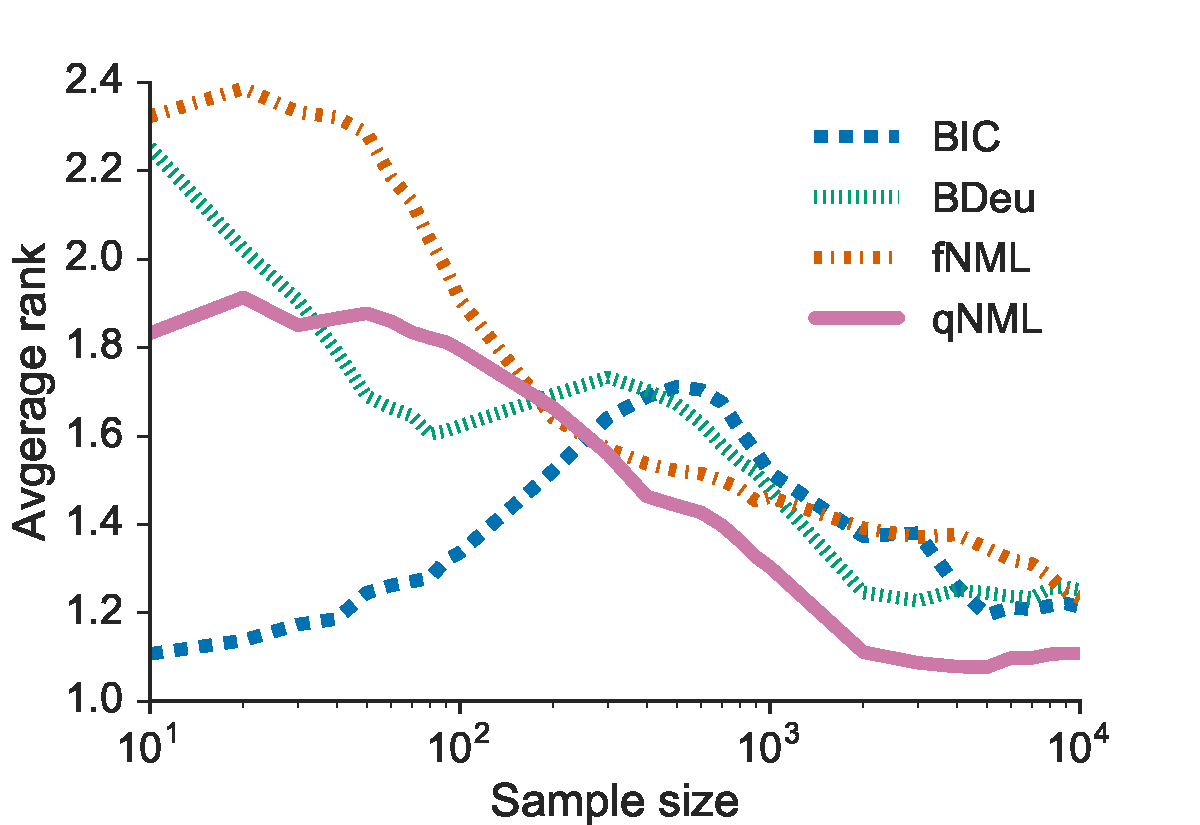
\includegraphics[width=8cm,height=5cm]{qNML_images/shd_rank_all.pdf}
\caption{Average ranks for the scoring functions in structure learning experiments.}
\label{fig:shd_ranks}
\end{figure}


%Not surprisingly, the results indicate that when the parameter generation
%mechanism matches the assumptions of the BDeu-score, BDeu usually
%also ranks the generating structure higher than the other scores (see Figure
%~\ref{fig:4arcs} and \ref{fig:7arcs}).  On the other hand, when the parameters are drawn from the
%Jeffreys' prior, the fNML score appears to rank the generating structure
%highest. This too is not surprising, since the NML distribution for
%multinomial data is known to closely match the marginal distribution of
%the data when the Jeffreys' prior is used.
%
%The underfitting tendency of BIC can also be clearly detected both for
%relatively sparse networks (4 arcs) and for dense ones (7 arcs). The
%ranking ability of the qNML criterion appears to be between
%fNML and BDeu in 3 out of 4 settings which is good considering that
%one of these criteria is always the winner. For dense networks with
%the BDeu prior, qNML appears to perform worse than BDeu and fNML but
%still much better than BIC.

\subsection{Prediction and Parsimony}

To empirically compare the model selection criteria, we took 20 UCI
data sets~\cite{Lichman:2013} and ran train and test experiments for
all of them. To better compare the performance over different sample
sizes, we picked different fractions ($10\%, 20\%, \ldots, 90\%$) of
the data sets as training data and the rest as the test data.
This was done for 1000 different permutations of each data set.
The training was conducted using the dynamic
programming based exact structure learning algorithm.

When predicting $P(d_{test}|D_{train},S,\theta)$
with structures $S$ learned by the BDeu score, we used the
Bayesian predictive parameter values (BPP) $\theta_{ijk} \propto
N_{ijk}+\frac{1}{r_iq_i}$.  In the spirit of keeping the scores
hyperparameter-free, for structures learned by the other model
selection criteria, we used the sequential predictive NML (sNML)
parametrization $\theta_{ijk}\propto e(N_{ijk})(N_{ijk}+1)$, where
$e(n)=(\frac{n+1}{n})^n$ as suggested in~\cite{Riss07b}.

\begin{table}
\caption{Average predictive performance rank over different sample sizes for different model selection criteria in 20 different data sets.}
\label{tbl:preds}
\begin{center}
\begin{tabular}{crrrrr}
       Data
    & N
    & \multicolumn{1}{p{0.7cm}}{\centering BDeu \\ BPP}
    & \multicolumn{1}{p{0.8cm}}{\centering BIC \\ sNML}
    & \multicolumn{1}{p{0.9cm}}{\centering fNML \\ sNML}
    & \multicolumn{1}{p{0.9cm}}{\centering qNML \\ sNML}\\
       \midrule
 PostOpe &     90 &              2.79 &     \textbf{1.20} &  \underline{3.06} &           2.94 \\
    Iris &    150 &  \underline{2.82} &              2.37 &     \textbf{2.27} &           2.54 \\
    Wine &    178 &  \underline{3.23} &     \textbf{1.88} &              2.67 &           2.22 \\
   Glass &    214 &  \underline{3.61} &              3.09 &     \textbf{1.42} &           1.88 \\
 Thyroid &    215 &              2.55 &  \underline{3.21} &     \textbf{1.80} &           2.44 \\
 HeartSt &    270 &  \underline{3.12} &     \textbf{1.39} &              3.12 &           2.37 \\
 BreastC &    286 &  \underline{3.09} &     \textbf{1.41} &              2.97 &           2.53 \\
 HeartHu &    294 &  \underline{3.18} &     \textbf{1.66} &              2.90 &           2.27 \\
 HeartCl &    303 &  \underline{3.46} &     \textbf{1.38} &              2.99 &           2.17 \\
   Ecoli &    336 &              3.20 &  \underline{3.53} &     \textbf{1.24} &           2.04 \\
   Liver &    345 &  \underline{3.17} &              2.39 &              2.69 &  \textbf{1.75} \\
 Balance &    625 &  \underline{3.35} &              1.91 &     \textbf{1.59} &           3.16 \\
 BcWisco &    699 &  \underline{3.06} &              2.03 &              2.89 &  \textbf{2.02} \\
 Diabete &    768 &  \underline{2.91} &              2.70 &              2.68 &  \textbf{1.71} \\
 TicTacT &    958 &  \underline{3.44} &              2.71 &     \textbf{1.31} &           2.53 \\
   Yeast &   1484 &              2.60 &  \underline{3.76} &     \textbf{1.55} &           2.10 \\
 Abalone &   4177 &              2.60 &  \underline{3.64} &     \textbf{1.04} &           2.72 \\
 PageBlo &   5473 &              2.24 &  \underline{3.61} &     \textbf{1.31} &           2.83 \\
   Adult &  32561 &              3.23 &  \underline{3.77} &     \textbf{1.00} &           2.00 \\
 Shuttle &  58000 &     \textbf{1.44} &  \underline{3.78} &              1.56 &           3.22 \\
\end{tabular}
\end{center}
\end{table}

For each train/test sample, we ranked the predictive performance of
the models learned by the four different scores (rank
1 being the best and 4 the worst). Table~\ref{tbl:preds} features the
average rank for different data sets, the average being taken over
1000 different train/test samples for each 9 sample sizes.
BIC's bias for simplicity makes it often win (written bold in
the table) with small sample sizes, but it performs worst
(underlined) for the larger sample sizes (for the same reason), while
fNML seems to be good for large sample sizes. The striking feature
about the qNML is its robustness.  It is usually between BIC and fNML
for all the sample sizes making it a ``safe choice''. This can be
quantified if we further average the columns of
Table~\ref{tbl:preds}, yielding the average ranks of $2.95, 2.57,
2.10$, and $2.37$, with standard deviations $0.49, 0.90, 0.76$, and
$0.43$.  While fNML achieves on average the best rank, the runner-up
qNML has the lowest standard deviation.

Figure~\ref{fig:bcnpmean} shows how fNML still sometimes behaves
strangely in terms of model complexity as measured by the number of
parameters in the model. qNML, instead, appears to yield more
parsimonious models. To study the concern of fNML producing too
complex models for small sample sizes, we studied the number of
parameters in models produced by different scores when using
10\% of each data set for structure learning.

Looking at the number of parameters for the same 20 data sets again
features BIC's preference for simple models
(Table~\ref{tbl:nofparams}).  qNML usually (19/20) yields more
parsimonious models than fNML that selects the most complex model for
7 out of 20 data sets.

The graphs for different sample sizes for both predictive accuracy and
the number of parameters can be found in Appendix E in the Supplementary Material.

\begin{table}
  \caption{Average number of parameters in models 
    for different scores in 20 different data sets.}
\label{tbl:nofparams}
\begin{center}
\begin{tabular}{crrrrr}
%%    Data &     N &              BDeu &               BIC &           fNML &              qNML \\
       Data
    & N
    & \multicolumn{1}{p{0.7cm}}{\centering BDeu\\ }
    & \multicolumn{1}{p{0.8cm}}{\centering BIC\\ }
    & \multicolumn{1}{p{0.9cm}}{\centering fNML\\}
    & \multicolumn{1}{p{0.9cm}}{\centering qNML\\}\\
\midrule
    Iris &    15 &     \underline{37} &   \textbf{23} &                33 &               29 \\
 PostOpe &    18 &   \underline{1217} &   \textbf{19} &               397 &              146 \\
   Ecoli &    34 &    \underline{182} &   \textbf{31} &               162 &               77 \\
   Liver &    35 &                 45 &   \textbf{15} &    \underline{61} &               24 \\
    Wine &    36 &  \underline{16521} &   \textbf{70} &               807 &              205 \\
   Glass &    44 &   \underline{1677} &   \textbf{48} &               506 &               97 \\
 Thyroid &    44 &                 40 &   \textbf{23} &    \underline{66} &               28 \\
 HeartSt &    54 &  \underline{16861} &   \textbf{44} &              1110 &              256 \\
 BreastC &    58 &  \underline{25797} &   \textbf{49} &              3767 &              844 \\
 HeartHu &    60 &   \underline{1634} &   \textbf{43} &               792 &               90 \\
 HeartCl &    62 &  \underline{34381} &   \textbf{47} &              1433 &              404 \\
 BcWisco &    70 &   \underline{4630} &   \textbf{42} &               603 &               89 \\
 Diabete &    77 &                 39 &   \textbf{22} &   \underline{216} &               34 \\
 TicTacT &    96 &  \underline{13701} &   \textbf{25} &              1969 &              767 \\
 Balance &   126 &        \textbf{20} &            24 &                49 &  \underline{611} \\
   Yeast &   149 &                 71 &   \textbf{31} &   \underline{265} &               75 \\
 Abalone &   418 &                 91 &   \textbf{46} &   \underline{150} &               63 \\
 PageBlo &   548 &    \underline{703} &   \textbf{45} &               380 &               56 \\
 Shuttle &  5800 &                535 &   \textbf{99} &   \underline{717} &              130 \\
   Adult &  6513 &                699 &  \textbf{479} &  \underline{1555} &              945 \\
\end{tabular}
\end{center}
\end{table}
